\documentclass[a4paper]{oblivoir}
\usepackage{amsmath,amssymb,kotex,kswrapfig,mdframed,tabto,paralist,graphicx,enumitem}
\usepackage{fapapersize}
\usefapapersize{210mm,297mm,10mm,*,10mm,*}

%%% Counters
\newcounter{num}

%%% Commands
\newcommand\defi[1]
{\bigskip\par\noindent\stepcounter{num} \textbf{정의 \thenum) #1}\par\noindent}
\newcommand\theo[1]
{\bigskip\par\noindent\stepcounter{num} \textbf{정리 \thenum) #1}\par\noindent}
\newcommand\exam[1]
{\bigskip\par\noindent\stepcounter{num} \textbf{예시 \thenum) #1}\par\noindent}
\newcommand\prob[1]
{\bigskip\par\noindent\stepcounter{num} \textbf{문제 \thenum) #1}\par\noindent}

\newcommand\pb[1]{\ensuremath{\fbox{\phantom{#1}}}}

\newcommand\ba{\ensuremath{\:|\:}}

\newcommand\procedure[1]{\begin{mdframed}\vspace{#1\textheight}\end{mdframed}\bigskip}

\newcommand\an[1]{\bigskip\par\noindent\textbf{문제 #1)}\par\noindent}

%%% Meta Commands
\let\oldsection\section
\renewcommand\section{\clearpage\oldsection}

\let\emph\textsf

%%% Title
\title{그래프 그리기 (가우스 함수)}
\date{\today}
\author{}

\begin{document}
\maketitle

\noindent
다음 함수에 대하여 불연속 점의 개수를 구하여라.
\begin{enumerate}[label = (\arabic*)]%, itemsep = 0pt]
\item
\(y=[x]\quad(-4\le x\le4)\)
\item
\(y=[2x+1]\quad(-2\le x\le2)\)
\item
\(y=[\frac12x+1]\quad(-4\le x\le4)\)
\item
\(y=[x^2]\quad(-2\le x\le2)\)
\item
\(y=[\frac12x^2-4]\quad(-4\le x\le4)\)
\end{enumerate}

\bigskip\bigskip\bigskip\bigskip
\begin{minipage}{0.45\textwidth}\centering
\(y=x\quad(-4\le x\le4)\)
\par\bigskip\includegraphics[width=0.9\textwidth]{55}
\end{minipage}
\begin{minipage}{0.45\textwidth}\centering
\(y=[x]\quad(-4\le x\le4)\)
\par\bigskip\includegraphics[width=0.9\textwidth]{55}
\end{minipage}\bigskip\bigskip\par
\begin{minipage}{0.45\textwidth}\centering
\(y=2x+1\quad(-2\le x\le2)\)
\par\bigskip\includegraphics[width=0.9\textwidth]{55}
\end{minipage}
\begin{minipage}{0.45\textwidth}\centering
\(y=[2x+1]\quad(-2\le x\le2)\)
\par\bigskip\includegraphics[width=0.9\textwidth]{55}
\end{minipage}\bigskip\bigskip\par

\newpage
\begin{minipage}{0.45\textwidth}\centering
\(y=\frac12x+1\quad(-4\le x\le4)\)
\par\bigskip\includegraphics[width=0.9\textwidth]{55}
\end{minipage}
\begin{minipage}{0.45\textwidth}\centering
\(y=[\frac12x+1]\quad(-4\le x\le4)\)
\par\bigskip\includegraphics[width=0.9\textwidth]{55}
\end{minipage}\bigskip\bigskip\par
\begin{minipage}{0.45\textwidth}\centering
\(y=x^2\quad(-2\le x\le2)\)
\par\bigskip\includegraphics[width=0.9\textwidth]{55}
\end{minipage}
\begin{minipage}{0.45\textwidth}\centering
\(y=[x^2]\quad(-2\le x\le2)\)
\par\bigskip\includegraphics[width=0.9\textwidth]{55}
\end{minipage}\bigskip\bigskip\par
\begin{minipage}{0.45\textwidth}\centering
\(y=\frac12x^2-4\quad(-4\le x\le4)\)
\par\bigskip\includegraphics[width=0.9\textwidth]{55}
\end{minipage}
\begin{minipage}{0.45\textwidth}\centering
\(y=[\frac12x^2-4]\quad(-4\le x\le4)\)
\par\bigskip\includegraphics[width=0.9\textwidth]{55}
\end{minipage}\bigskip\bigskip\par

%%
\section*{답}
\begin{enumerate}[label = (\arabic*)]%, itemsep = 0pt]
\item
8
\item
8
\item
4
\item
8
\item
16
\end{enumerate}

\begin{minipage}{0.45\textwidth}\centering
\(y=x\quad(-4\le x\le4)\)
\par\bigskip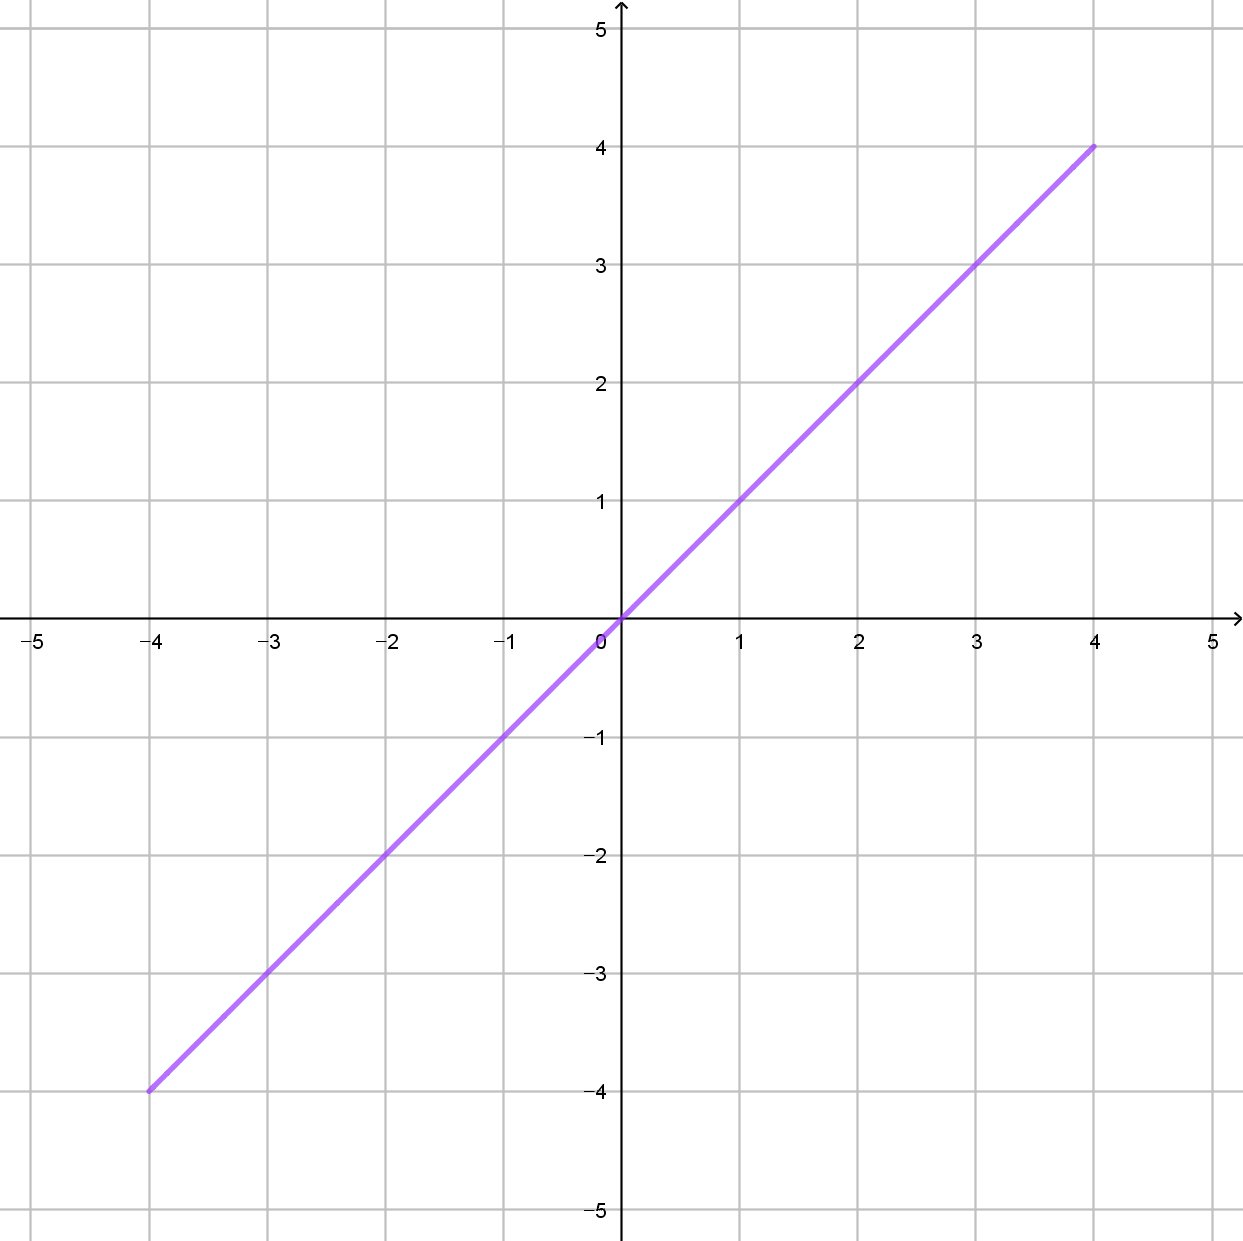
\includegraphics[width=0.9\textwidth]{img/y=x}
\end{minipage}
\begin{minipage}{0.45\textwidth}\centering
\(y=[x]\quad(-4\le x\le4)\)
\par\bigskip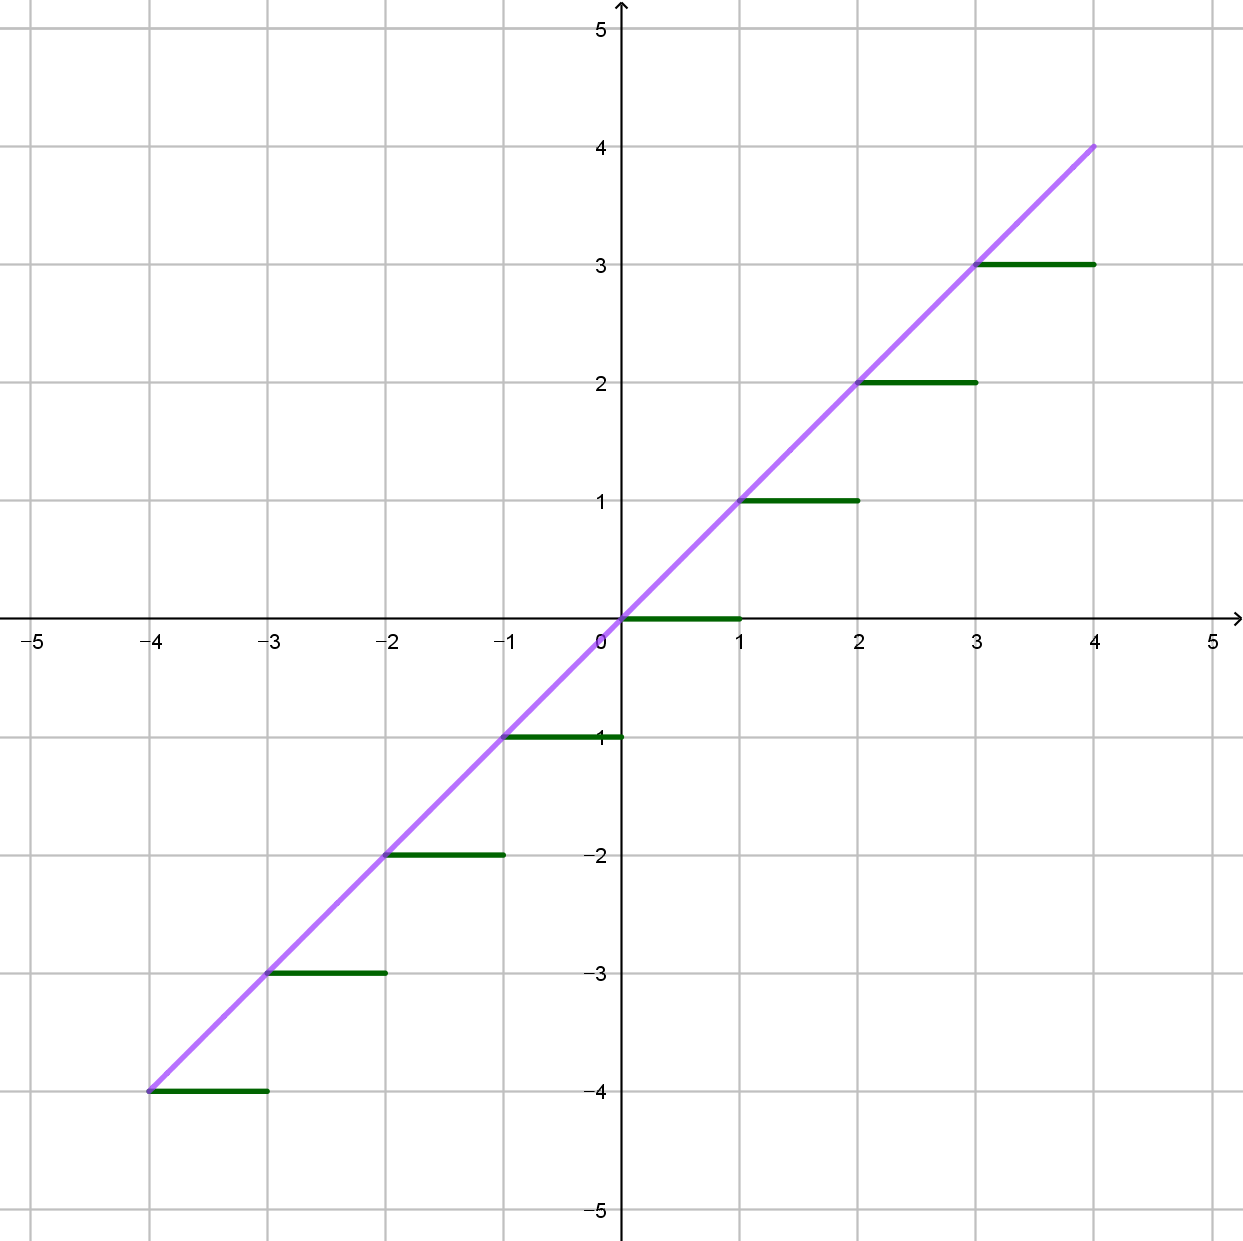
\includegraphics[width=0.9\textwidth]{img/y=[x]}
\end{minipage}\bigskip\bigskip\par
\begin{minipage}{0.45\textwidth}\centering
\(y=2x+1\quad(-2\le x\le2)\)
\par\bigskip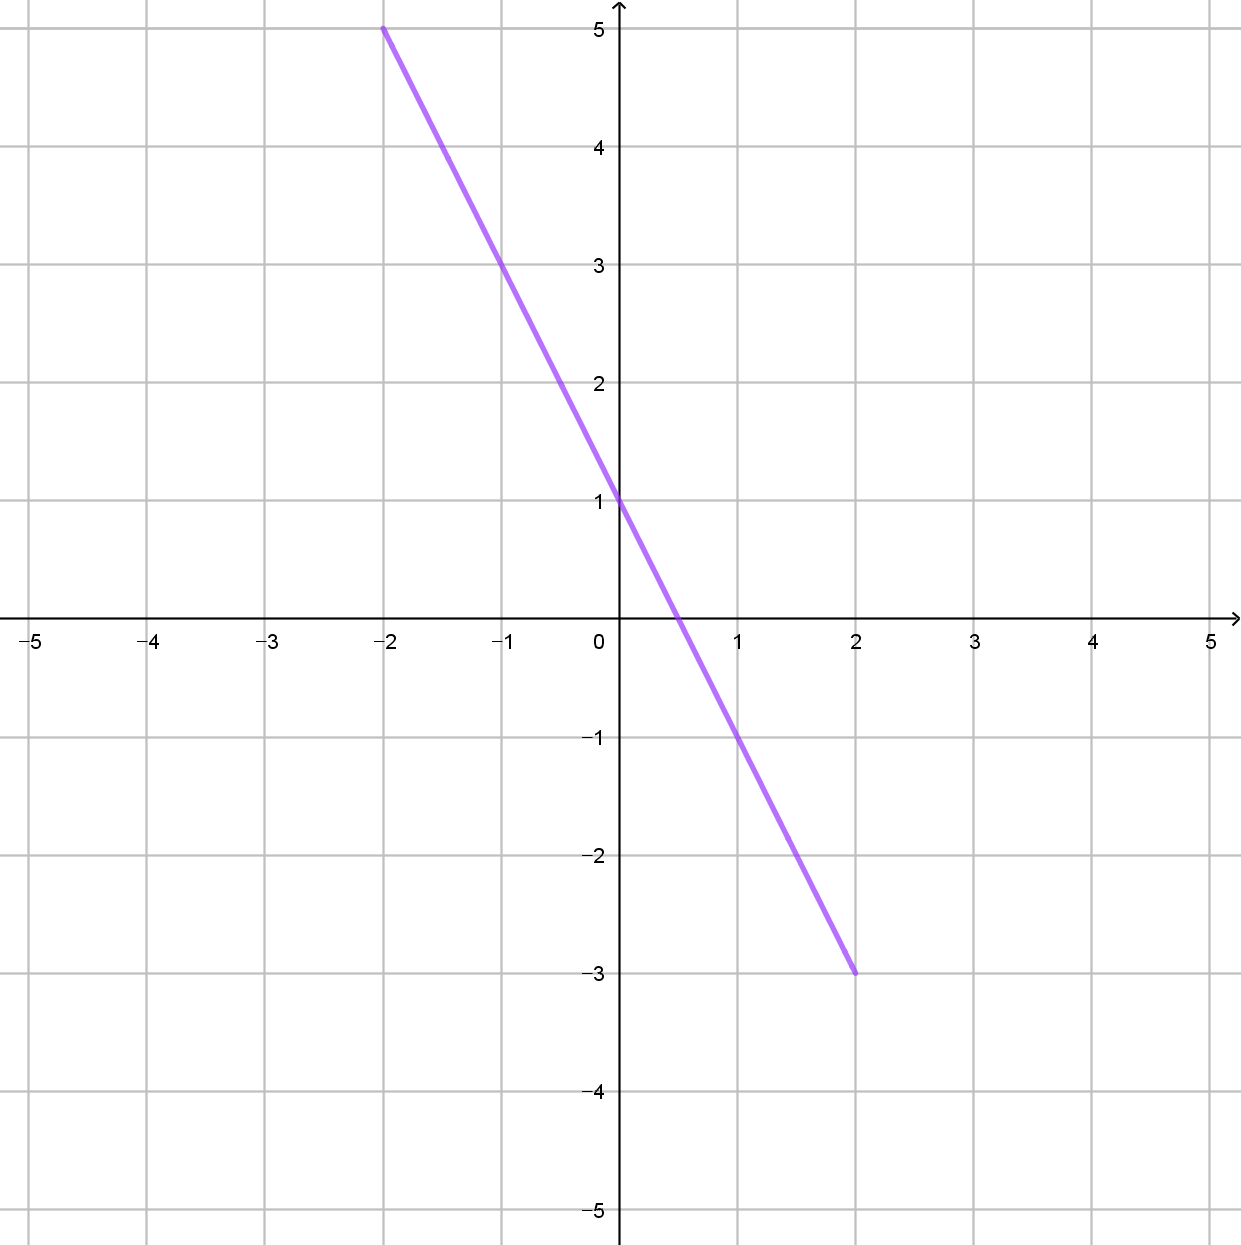
\includegraphics[width=0.9\textwidth]{img/y=-2x+1}
\end{minipage}
\begin{minipage}{0.45\textwidth}\centering
\(y=[2x+1]\quad(-2\le x\le2)\)
\par\bigskip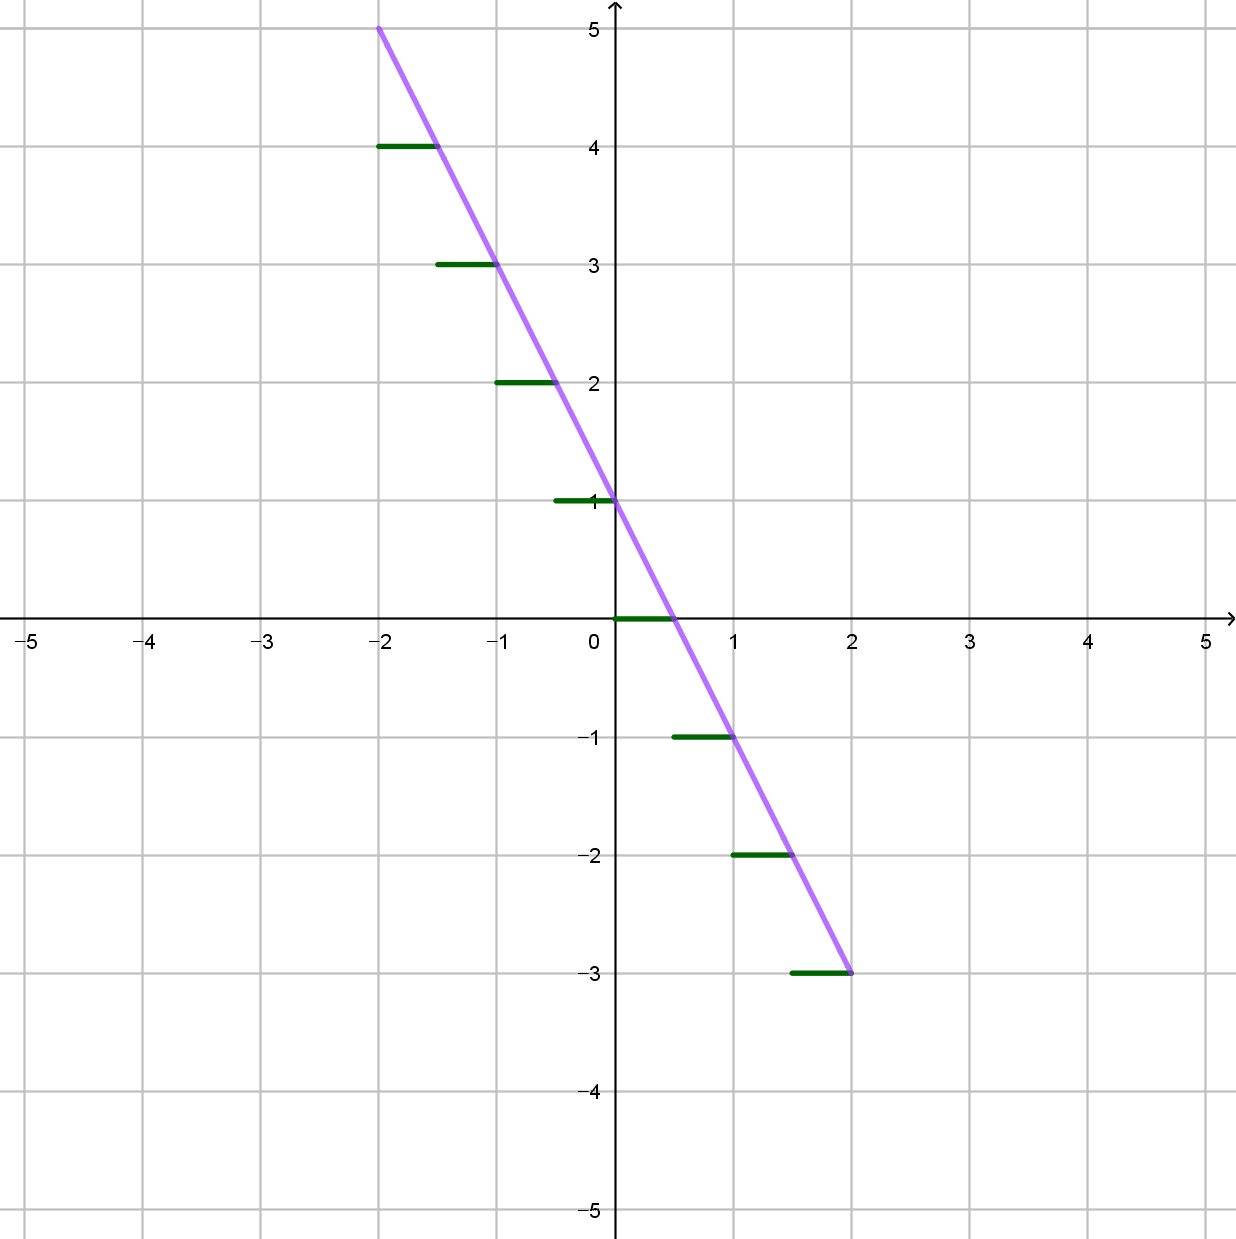
\includegraphics[width=0.9\textwidth]{img/y=[-2x+1]}
\end{minipage}\bigskip\bigskip\par

\newpage
\begin{minipage}{0.45\textwidth}\centering
\(y=\frac12x+1\quad(-4\le x\le4)\)
\par\bigskip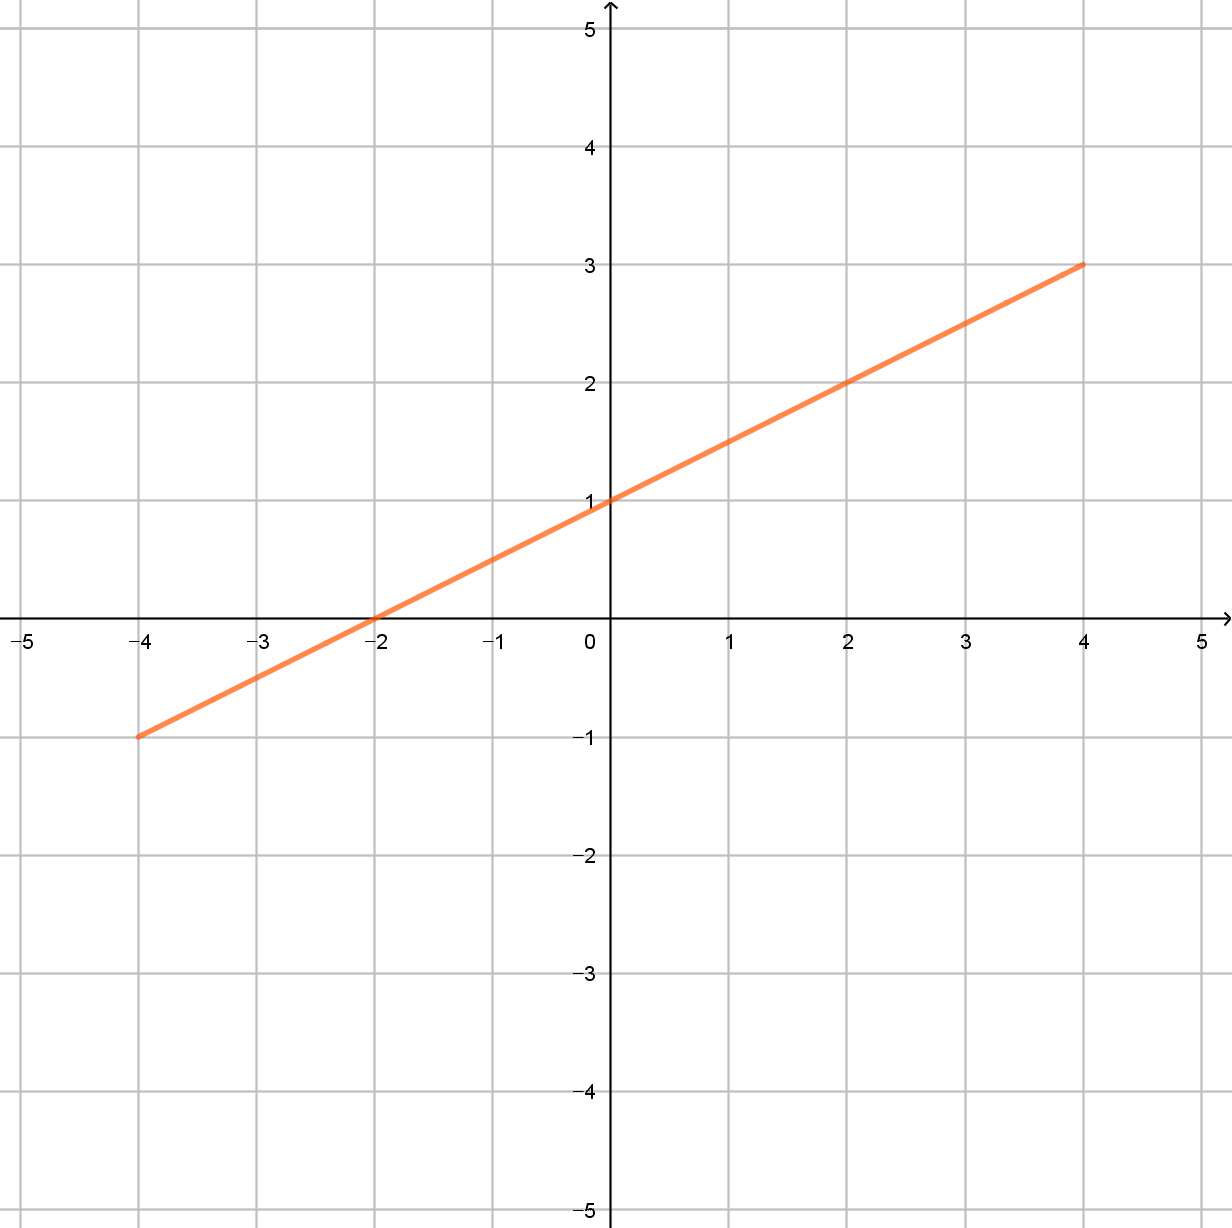
\includegraphics[width=0.9\textwidth]{img/y=.5x+1}
\end{minipage}
\begin{minipage}{0.45\textwidth}\centering
\(y=[\frac12x+1]\quad(-4\le x\le4)\)
\par\bigskip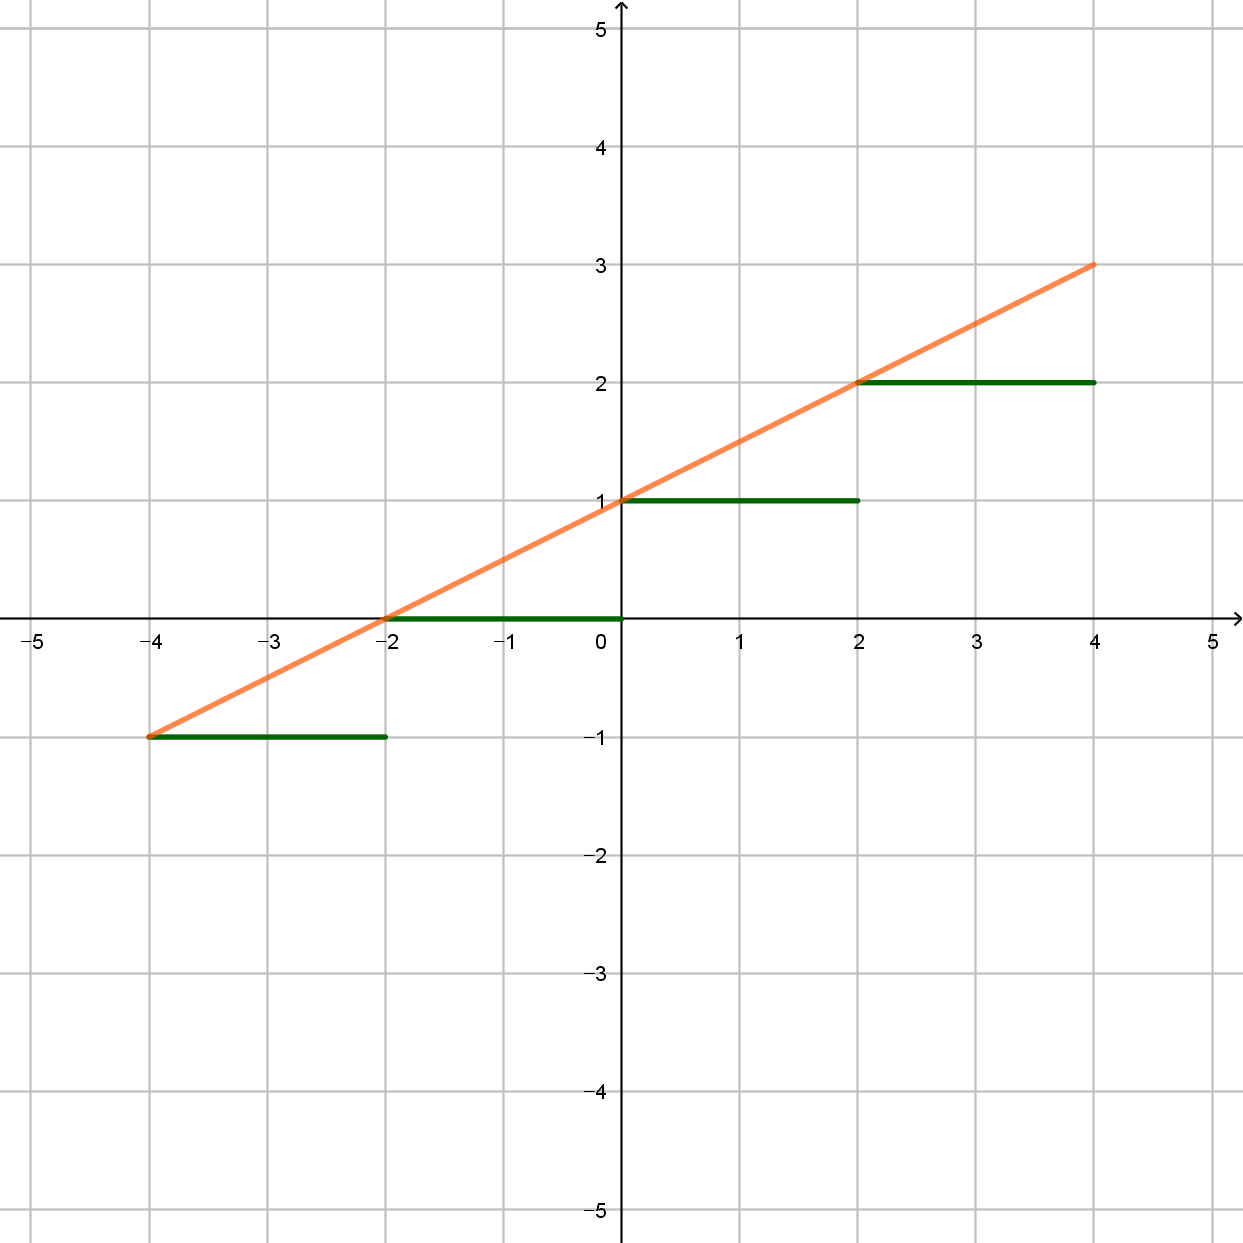
\includegraphics[width=0.9\textwidth]{img/y=[.5x+1]}
\end{minipage}\bigskip\bigskip\par
\begin{minipage}{0.45\textwidth}\centering
\(y=x^2\quad(-2\le x\le2)\)
\par\bigskip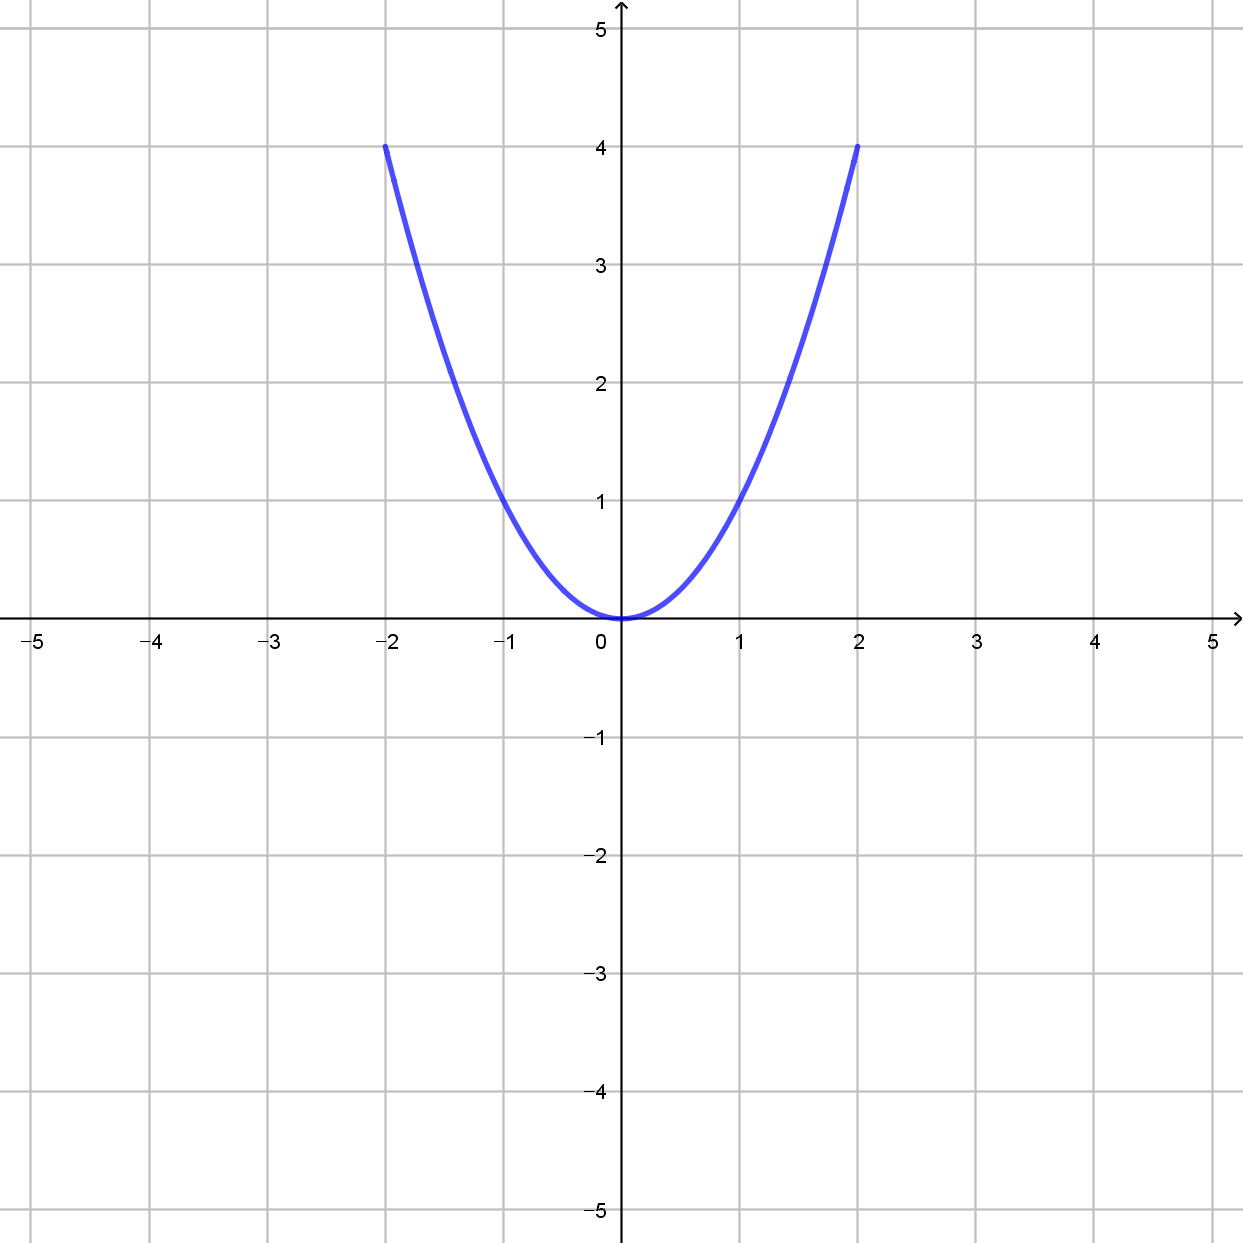
\includegraphics[width=0.9\textwidth]{img/y=x^2}
\end{minipage}
\begin{minipage}{0.45\textwidth}\centering
\(y=[x^2]\quad(-2\le x\le2)\)
\par\bigskip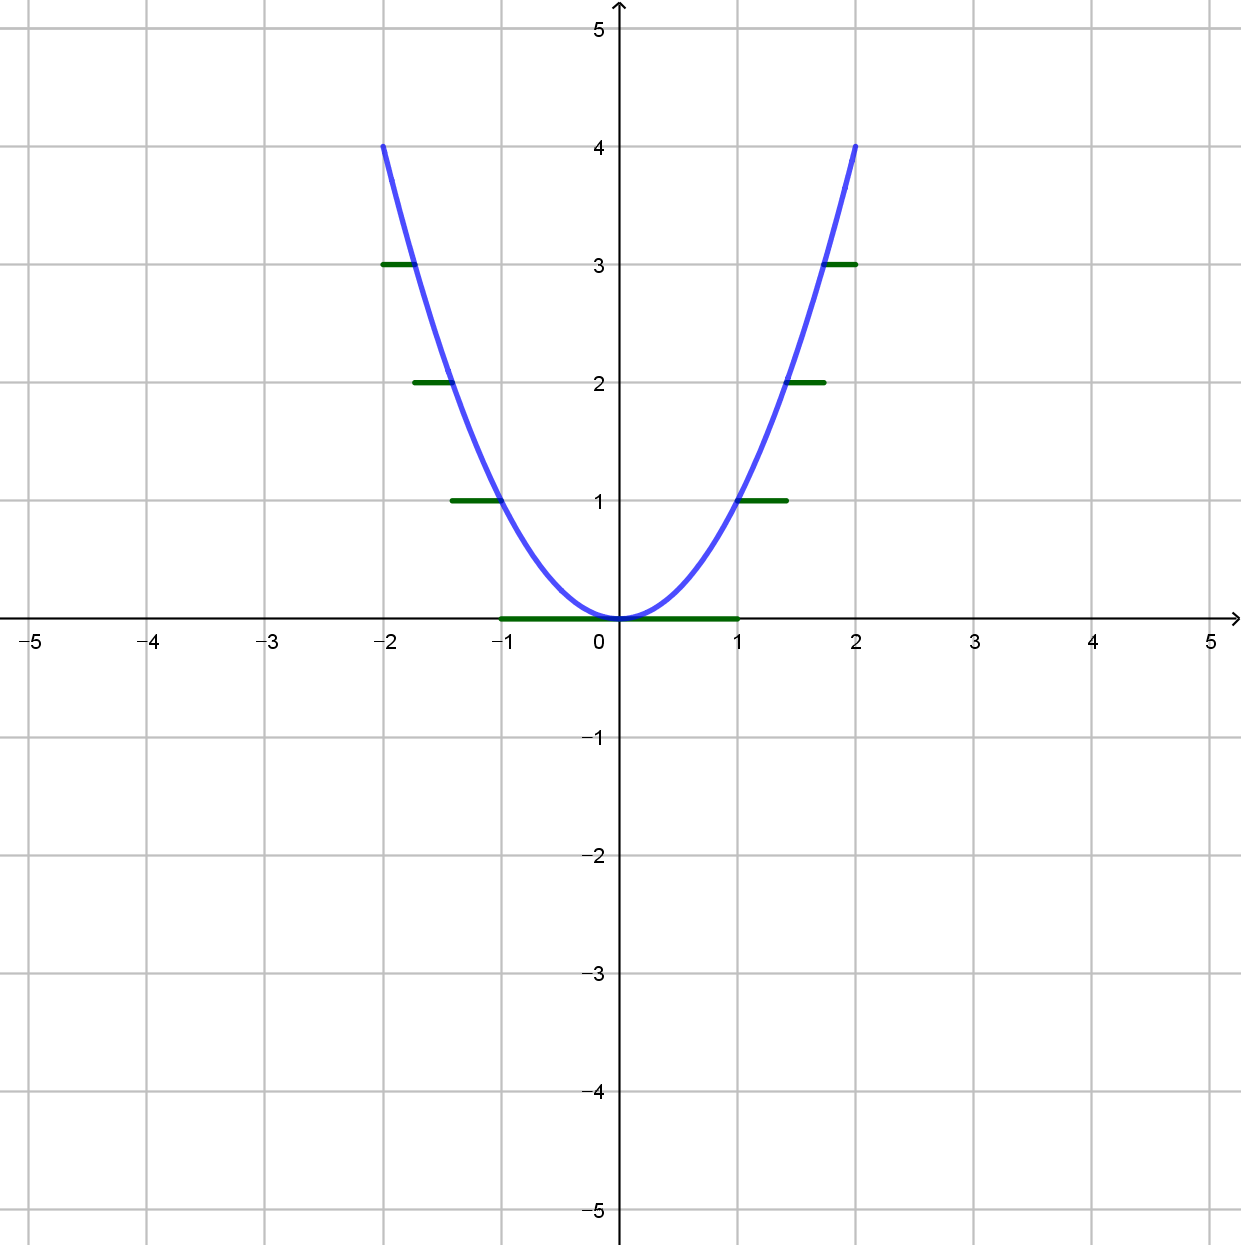
\includegraphics[width=0.9\textwidth]{img/y=[x^2]}
\end{minipage}\bigskip\bigskip\par
\begin{minipage}{0.45\textwidth}\centering
\(y=2x^2-1\quad(-4\le x\le4)\)
\par\bigskip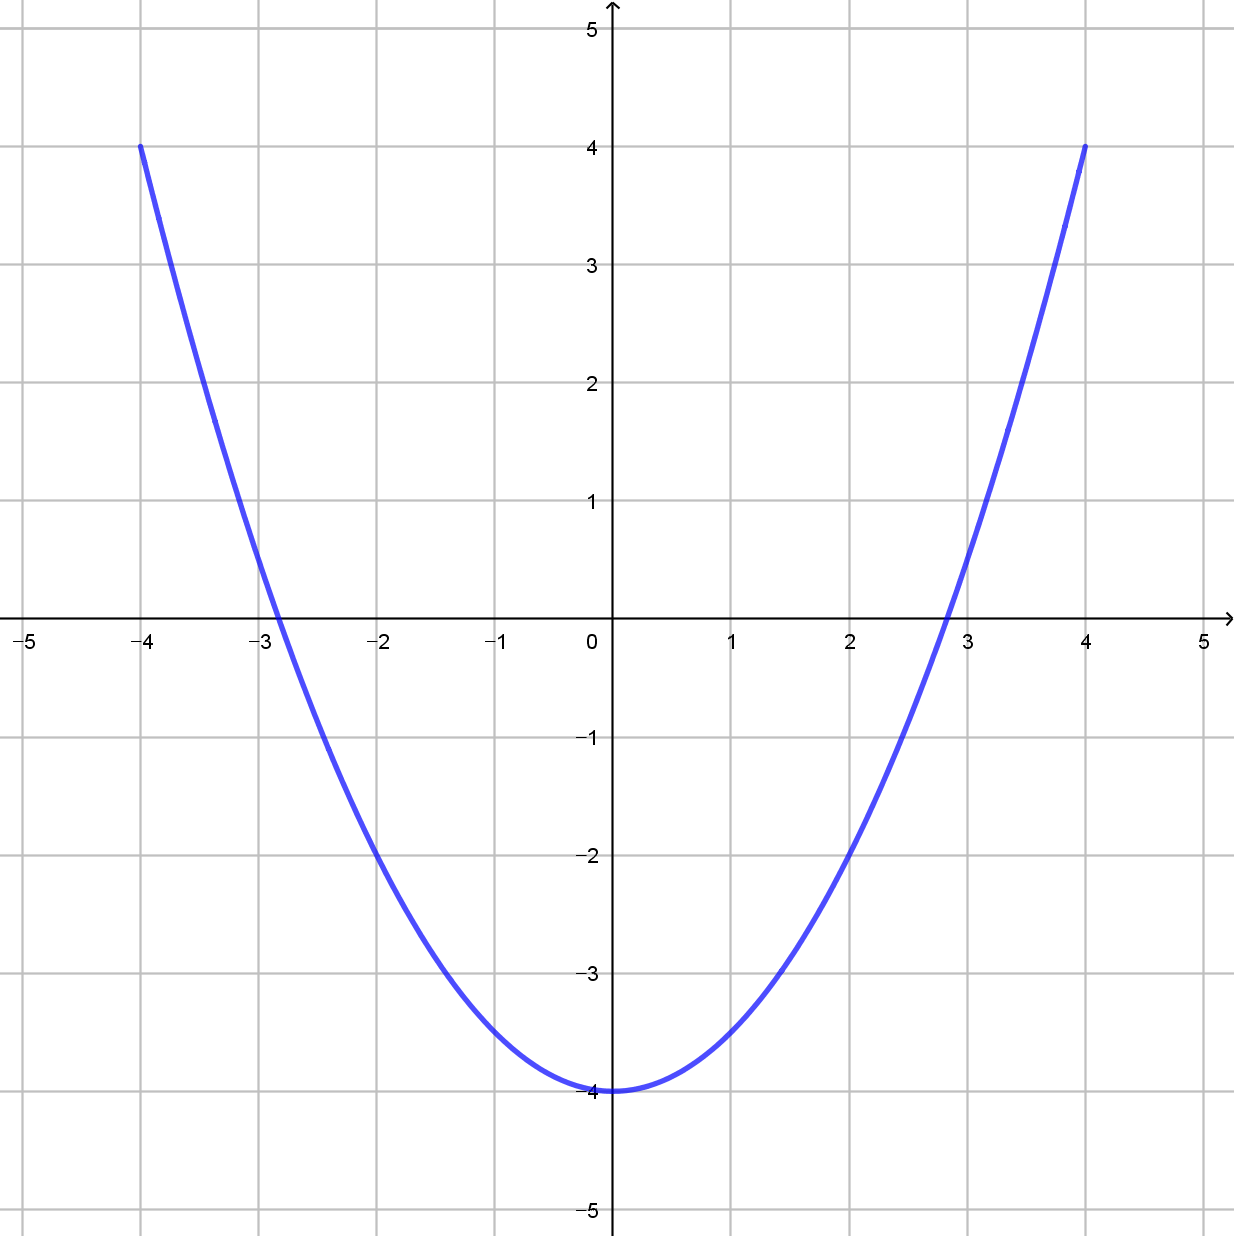
\includegraphics[width=0.9\textwidth]{img/y=.5x^2-4}
\end{minipage}
\begin{minipage}{0.45\textwidth}\centering
\(y=[2x^2-1]\quad(-4\le x\le4)\)
\par\bigskip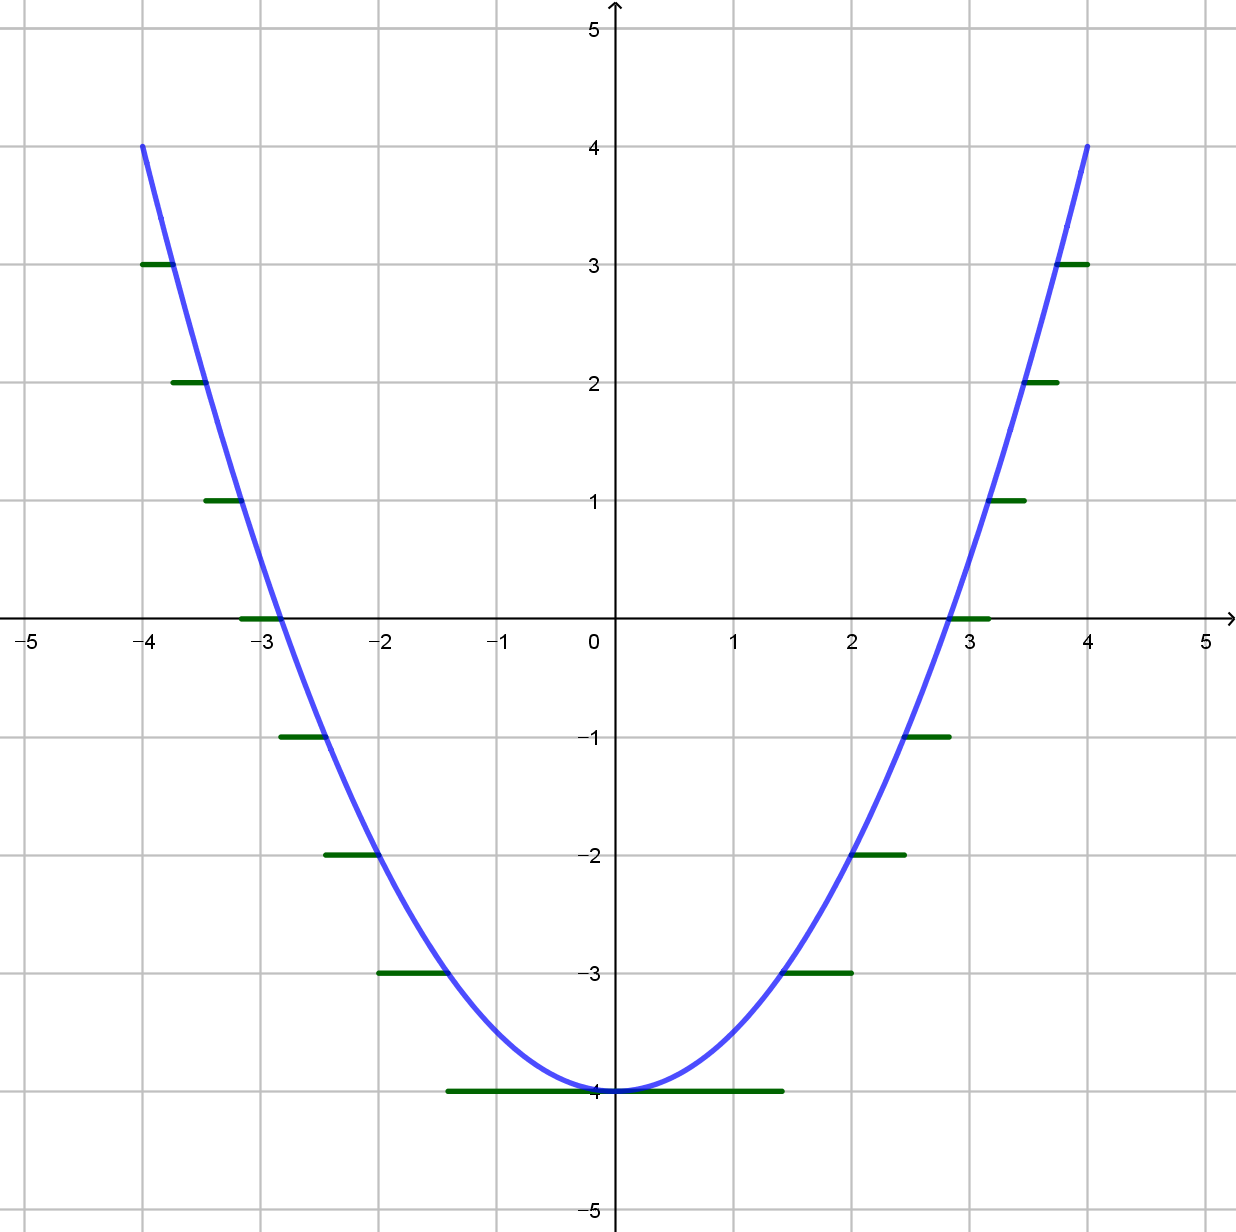
\includegraphics[width=0.9\textwidth]{img/y=[.5x^2-4]}
\end{minipage}\bigskip\bigskip\par

\end{document}